% The jmlr pmlr option provides the L4DC format.
% References are maintained in references.bib.
\documentclass[pmlr]{jmlr}
\usepackage[T1]{fontenc}
\usepackage{times}
\usepackage{amsmath,amssymb,booktabs}
\usepackage{afterpage}

\title[$\alpha$-PLAYER: Game-Theoretic Robot Table Tennis]{
  $\alpha$-PLAYER: An Attacker--Defender Framework for
  Game-Theoretic Planning and Learning in Robot Table Tennis}
\author{\Name{Anonymous Authors}}
\jmlryear{2027}
\jmlrvolume{--}
\jmlrworkshop{Learning for Dynamics and Control}
\editors{}

\newcommand{\Players}{\mathcal{N}}
\newcommand{\States}{\mathcal{X}}
\newcommand{\Actions}{\mathcal{A}}
\newcommand{\E}{\mathbb{E}}
\newcommand{\R}{\mathbb{R}}
\newcommand{\ind}{\mathbf{1}}
\newcommand{\attack}{\mathrm{A}}
\newcommand{\defend}{\mathrm{D}}
\newcommand{\resultblank}{\phantom{0.00}}

\begin{document}
\maketitle

\begin{abstract}
Competitive robot table tennis extends beyond the challenge of controlling a robot at its physical limits. Like human players, robots must choose where to return the ball and how to prepare for the opponent's next shot to gain a strategic advantage. Despite recent advances in robot table tennis, research on equilibrium-aware planning for competitive play remains limited. We propose an algorithmic framework for computing approximate Nash equilibrium strategies by adapting dynamic $\alpha$-potential functions to robot table tennis.
We introduce a table tennis environment organized around an attacker--defender game: the attacker returns the ball, the defender prepares to receive it, and the roles switch when the returned ball crosses the net.
We also formulate self-play reinforcement learning over the same game. We evaluate both approaches and relevant baselines using robots with a high number of degrees of freedom in MuJoCo, measuring competitive win rates and unilateral response gains.
\end{abstract}

\begin{keywords}
Robot Table Tennis, Dynamic Games, Attacker--Defender Games,
Nash Equilibrium, $\alpha$-Potential Functions, Self-Play Reinforcement Learning.
\end{keywords}

% Queue the overview after page 1 so it appears at the top of page 2.
\afterpage{%
\begin{figure}[!t]
\centering
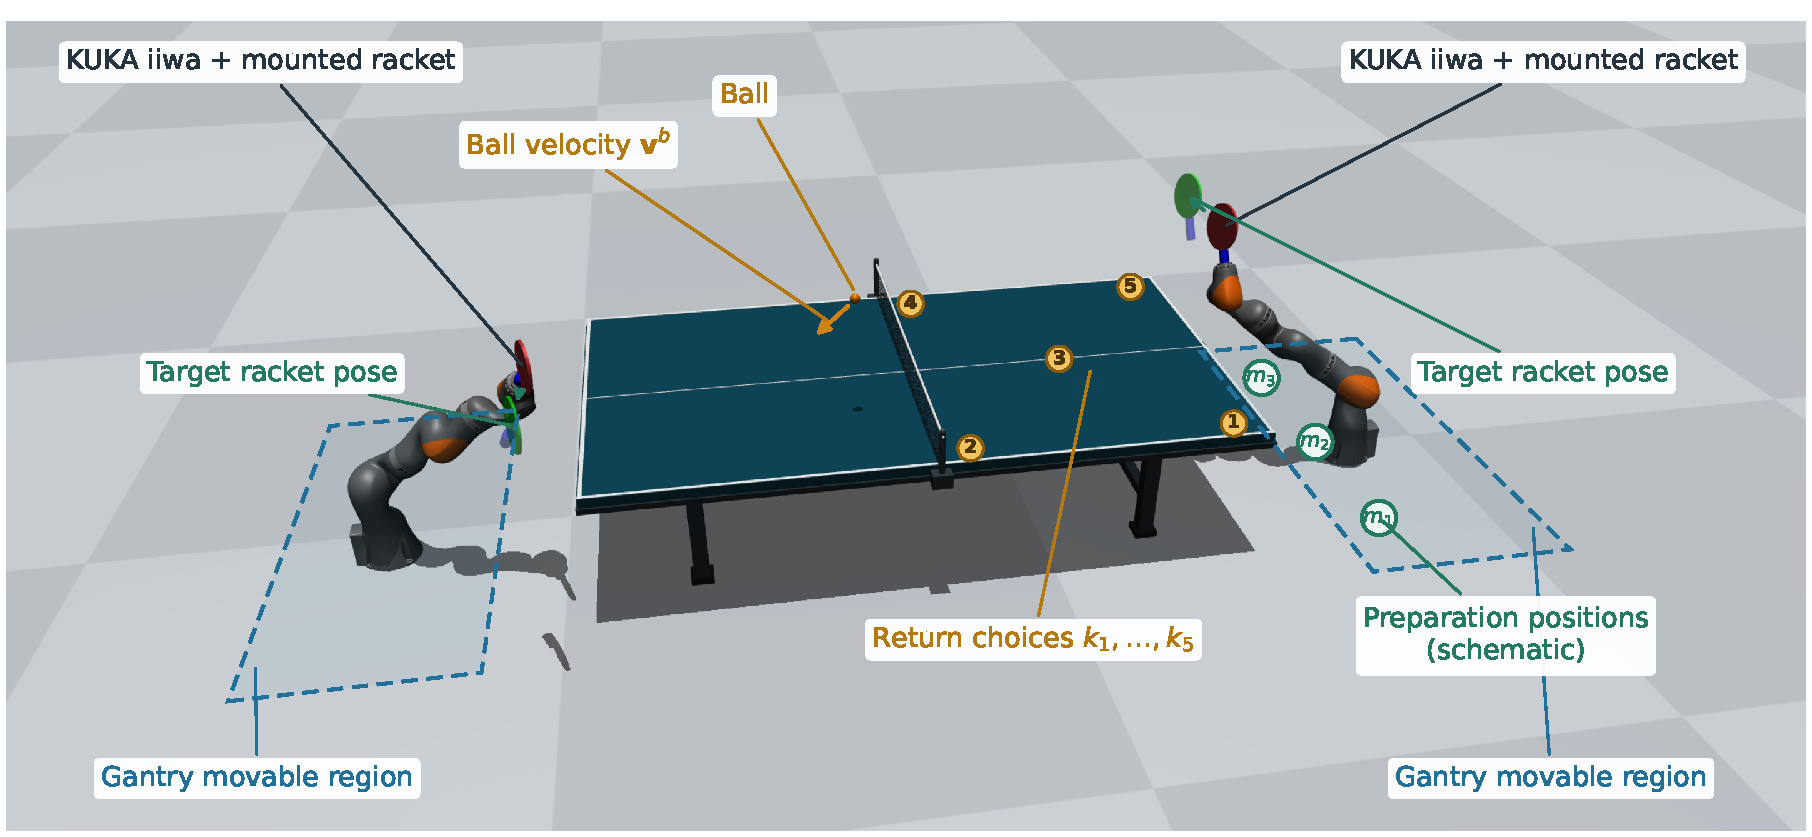
\includegraphics[width=\linewidth]{Figures/figure1.pdf}
\caption{Robot table-tennis game environment. Five return choices are marked on the right half of the table, with target 3 centered between the four corner targets. The preparation positions are marked for the right robot.}
\label{fig:environment}
\end{figure}
}

\section{Introduction}
\label{sec:introduction}

Table tennis provides a demanding setting for studying learning and control in interactive physical systems. A robot must estimate a moving ball, coordinate a rapid racket motion, and execute a legal return under its actuation and workspace constraints. Recent systems demonstrate substantial progress in competitive play against humans \citep{dambrosio2024competitive,durr2026ace}, while humanoid systems show that table tennis can be integrated with coordinated whole-body motion \citep{su2025hitter}. These advances make it possible to study a further question: how should a physically capable robot choose its actions when its opponent is also making strategic decisions?

Winning a rally depends on more than the accuracy of an individual return. A player may direct the ball toward an exposed part of the opponent's court, induce a difficult recovery motion, or vary shot placement to avoid becoming predictable. At the same time, that player must recover to a position from which it can respond to the next shot. A return that immediately challenges the opponent may also leave the player poorly prepared for a counterattack. Consequently, shot placement and defensive preparation are coupled across successive exchanges. Treating the opponent only as a source of incoming trajectories does not capture this reciprocal dependence.

Game theory provides a framework for reasoning about such interactions. A Nash equilibrium describes a strategy profile for which no player can improve its expected utility through a unilateral change. In robot table tennis, this concept connects the choice of return targets with the opponent's preparation strategy and the continuation of the rally. However, computing equilibrium strategies directly in the space of high-dimensional robot controls is difficult: both players influence ball motion, robot configurations persist between shots, and the consequences of an action extend beyond the next contact.

We address these challenges through a table tennis game organized around alternating attacker and defender roles. During an exchange, the attacker is the player responsible for producing the next return; the defender is the opponent preparing to receive that return. Their roles switch when the returned ball crosses the net. This decomposition provides a common interface between strategic decisions and physical execution. It also exposes a compact set of interpretable choices: five locations at which to return the ball and three positions from which to prepare for the next incoming shot. The underlying robot controllers continue to react to the physical state while executing these choices.

Our equilibrium approximation approach builds on the dynamic $\alpha$-potential framework and its application to autonomous racing in $\alpha$-RACER \citep{guo2023markov,guo2024dynamic,kalaria2025racer}. Rather than repeatedly solving coupled robot-control problems online, we learn a scalar function from simulated interactions and optimize it over policy parameters. The learning objective relates changes in this function to changes in individual players' long-term utilities. We additionally study self-play reinforcement learning through the same attacker--defender interface, providing a complementary route to learning competitive strategies. This comparison separates the strategic formulation from the particular algorithm used to solve it.

Our framework comprises two components:

\paragraph{Modeling and environment.}
We introduce a MuJoCo table tennis environment with an explicit attacker--defender decomposition and robots with a high number of degrees of freedom \citep{todorov2012mujoco}. Alternating strategic roles are coupled with ball dynamics, racket contacts, robot motion, and point outcomes, providing a shared environment for competitive planning and learning.

\paragraph{Strategic planning and learning.}
We adapt $\alpha$-potential learning to table tennis: offline interaction data estimate unilateral utility changes, and online potential optimization selects approximate equilibrium parameters. We compare this planner with PPO self-play and relevant baselines using common observations, strategic actions, execution controllers, and evaluation objectives.

\paragraph{Organization.}
Section~\ref{sec:related} reviews related work in robot table tennis, competitive robotic games, and equilibrium approximation. Section~\ref{sec:model} introduces the dynamic-game preliminaries and the attacker--defender formulation. Section~\ref{sec:approximation} presents potential-based equilibrium approximation and self-play reinforcement learning. Section~\ref{sec:results} compares competitive performance and unilateral response gains, and examines training-data and discount-factor choices. Section~\ref{sec:conclusion} concludes the paper.

\section{Related Work}
\label{sec:related}

\paragraph{Robot table tennis.}
Robot table tennis research spans landing-point control \citep{li2015landing}, learned return policies \citep{gao2020modelfree}, elite competitive play \citep{durr2026ace}, and humanoid whole-body control \citep{su2025hitter}. A representative competitive system is that of \citet{dambrosio2024competitive}, which combines hierarchical skill execution with online opponent adaptation to play against humans. We focus on equilibrium-aware selection of return targets and preparation positions across a rally.

\paragraph{Opponent modeling, game-theoretic planning, and self-play.}
Prior table tennis work studies safe opponent exploitation and anticipatory preparation \citep{wang2011safe,wang2017anticipation}. Most directly related, \citet{mahjourian2018hierarchical} learn cooperative and adversarial strategies through hierarchical self-play, with strategic actions specifying striking targets and waiting positions. Game-theoretic planning also supports competitive ground and aerial racing \citep{wang2019racing,spica2020drone}, using nonlinear game solvers and hierarchical controllers \citep{fridovich2020ilqgames,zhu2024sqp,thakkar2024hierarchical}. Beyond robotics, self-play and population-based learning produce competitive strategies in board and imperfect-information games \citep{silver2018alphazero,heinrich2016nfsp,lanctot2017psro}. We build on these approaches through an alternating-role table tennis game that compares $\alpha$-potential planning and self-play using a common strategic interface.

\paragraph{Potential functions and equilibrium approximation.}
Potential formulations reduce interactive planning to a single optimization problem \citep{kavuncu2021potential,jia2023rapid}. Dynamic $\alpha$-potential functions allow bounded disagreement between potential changes and unilateral utility changes \citep{guo2023markov,guo2024dynamic}. Our main algorithmic precedent is $\alpha$-RACER \citep{kalaria2025racer}, which learns this function offline from simulated interactions and optimizes it online over policy parameters. We adapt that procedure to shot placement and preparation; its equilibrium accuracy depends on the potential approximation and optimization errors.

\section{Modeling Multi-player Robot Table Tennis}
\label{sec:model}

We first introduce the dynamic-game notation, following the policy-parameter perspective used in $\alpha$-RACER \citep{kalaria2025racer}. We then instantiate the game for robot table tennis. The notation permits multiple strategic players; the attacker--defender environment developed here concerns singles table tennis, with two players.

\subsection{Preliminaries on Dynamic Game Theory}
\label{sec:preliminaries}

We consider a dynamic game with player set $\Players=\{1,\ldots,N\}$. At strategic decision epoch $t\in\{0,1,\ldots\}$, the joint state is $x_t\in\States$. Player $i$ chooses an action $a_t^i\in\Actions^i(x_t)$, and the joint action is $a_t=(a_t^i)_{i\in\Players}$. The state evolves according to a transition kernel
\begin{equation}
  x_{t+1}\sim P(\cdot\mid x_t,a_t),
  \label{eq:transition}
\end{equation}
which includes the physical execution of the selected actions. Player $i$ receives a bounded utility $r^i(x_t,a_t,x_{t+1})$. A state-feedback policy $\pi_h^i(\cdot\mid x;\theta^i)$ maps the state to a distribution over actions at rollout exchange $h$, where $\theta^i\in\Theta^i$ parameterizes an admissible policy family. We write $\Theta=\prod_{i\in\Players}\Theta^i$, $\theta=(\theta^i)_{i\in\Players}$, and $\theta^{-i}$ for the parameters of every player except $i$.

For discount factor $\gamma\in[0,1)$, the value of player $i$ from initial state $x$ is
\begin{equation}
  V^i(x,\theta^i,\theta^{-i})=
  \E_{\theta}\!\left[\sum_{t=0}^{\infty}
  \gamma^t r^i(x_t,a_t,x_{t+1})\,\middle|\,x_0=x\right].
  \label{eq:value}
\end{equation}
The expectation accounts for policy randomization and transition uncertainty. The parameters specify the complete evaluated policy, including its first-exchange action and subsequent continuation rule. Policies can depend on the state and the rollout exchange index. A terminal state is absorbing and has zero subsequent utility, so a finite rally is included in this notation.

\begin{definition}[$\epsilon$-Nash equilibrium at an initial state]
For $x\in\States$ and $\epsilon\geq0$, a joint policy parameter $\theta^*\in\Theta$ is an $\epsilon$-Nash equilibrium at $x$ if
\begin{equation}
  V^i(x,\theta^{*,i},\theta^{*,-i})
  \geq V^i(x,\theta^i,\theta^{*,-i})-\epsilon,
  \quad \forall i\in\Players,\ \forall\theta^i\in\Theta^i.
  \label{eq:nash}
\end{equation}
When $\epsilon=0$, the profile is a Nash equilibrium at $x$.
\end{definition}

If Equation~\eqref{eq:nash} holds for every admissible initial state, the profile is an $\epsilon$-Nash equilibrium over those states within the specified policy family. Throughout, deviations are taken within the specified policy families. Thus, equilibrium quality concerns the modeled strategic choices and their execution, rather than every possible joint-level robot policy.

\subsection{Robot Table Tennis as an Attacker--Defender Game}
\label{sec:game}

\paragraph{Players and strategic roles.}
For singles table tennis, $\Players=\{1,2\}$. The attacker and defender are roles assigned to these players, rather than additional players. Let $\iota_t\in\Players$ denote the attacker during exchange $t$, and let $\jmath_t=3-\iota_t$ denote the defender. The attacker receives the currently incoming ball and is responsible for producing the next return. The defender, having produced the preceding shot, prepares to receive the attacker's forthcoming return. The terms refer to these responsibilities even when a shot is tactically conservative. Each robot consists of a KUKA iiwa arm with a racket mounted on its end effector and a base mounted on a drivable gantry (Figure~\ref{fig:environment}).

\paragraph{Exchange timing and role switching.}
An exchange begins when the incoming ball crosses the net toward the attacker. At this crossing, the state is sampled, the attacker selects a return target, and the defender selects a preparation position. The returned ball's next net crossing starts a new exchange with $(\iota_{t+1},\jmath_{t+1})=(\jmath_t,\iota_t)$. A failed return or invalid shot terminates the rally. Appendix~\ref{app:execution} details the exchange initialization and timing.

\paragraph{Joint state.}
The state is $x_t=(b_t,z_t^1,z_t^2,\iota_t,\ell_t)$, where $b_t=(p_t^b,v_t^b,\omega_t^b)$ contains the ball position, velocity, and spin. Each $z_t^i$ includes gantry and joint positions, velocities, and controller state. Racket poses follow from kinematics, and $\ell_t$ records contact, bounce, and terminal status. Both robot states retain the effects of recovery and preparation on subsequent returns.

\paragraph{Strategic actions and information.}
Let $\mathcal{K}=\{1,\ldots,5\}$ index the return targets and $\mathcal{M}=\{1,2,3\}$ index the preparation positions. At exchange $t$, the attacker selects $k_t\in\mathcal{K}$ and the defender selects $m_t\in\mathcal{M}$, giving joint strategic action $(k_t,m_t)$. Equivalently,
\begin{equation}
  \Actions^i(x_t)=
  \begin{cases}
    \mathcal{K}, & i=\iota_t,\\
    \mathcal{M}, & i=\jmath_t.
  \end{cases}
  \label{eq:actions}
\end{equation}
% what my code does is - every player's actual action set, every exchange, is the full product $\mathcal{K}\times\mathcal{M}$ — never role-gated down to just one factor. Or are we talking about Kexin's design that alternating attacker/defender here?
% Dvij: Yes correct, that is an implementation detail and I think that is fine, fundamentally what I am describing here is how the environment evolves and for that only K for attacker and M for defender matters
Both choices use the physical state available at the exchange boundary. The defender does not receive the attacker's newly selected target before choosing its preparation action. Subsequent low-level control can react to observed ball motion. This timing models preparation under uncertainty about the next shot, rather than granting the defender advance knowledge of its destination. Figure~\ref{fig:environment} illustrates the environment and the attack-target and preparation-position geometry.

\paragraph{Physical execution and transition dynamics.}
Fixed execution controllers translate strategic targets into state-feedback robot commands. An attack controller $\kappa^{\attack,i}$ attempts to return the incoming ball toward the selected landing target; a preparation controller $\kappa^{\defend,i}$ moves the robot toward the selected ready configuration. Appendix~\ref{app:execution} describes the low-level execution interface. MuJoCo advances the robot and ball dynamics, including the modeled table, net, and racket interactions \citep{todorov2012mujoco}. Together, the execution controllers and simulation define
\begin{equation}
  x_{t+1}\sim P_{\mathrm{TT}}(\cdot\mid x_t,k_t,m_t).
  \label{eq:ttkernel}
\end{equation}
The selected target is a command, not a guaranteed physical outcome. Actuation limits, incoming-ball conditions, and execution error can lead to a different landing point or a failed return. The transition therefore retains the physical difficulty of realizing a strategically desirable shot.

\paragraph{Utility and continuation.}
For a point-based competitive objective, we define
\begin{equation}
\begin{aligned}
  r^i(x_t,a_t,x_{t+1})={}&
  \ind\{\text{player }i\text{ wins the point on this transition}\}\\
  &-\ind\{\text{player }i\text{ loses the point on this transition}\}.
\end{aligned}
  \label{eq:reward}
\end{equation}
The utility is zero while the rally continues, and $r^1=-r^2$ for a resolved point. Equation~\eqref{eq:value} then values the discounted point outcome over the continuation of the rally. A discount below one gives greater weight to earlier outcomes; it is a modeling choice rather than the official scoring rule. The competitive objective rewards winning points, while legal return execution and preparation enter through the transition dynamics.

\paragraph{Policy parameterization.}
\label{sec:policy_param}
A complete strategy specifies attack and defense behavior because each player occupies both roles. Self-play RL represents these behaviors with neural categorical policies. For $\alpha$-potential planning, the parameters specify only the current attack target and preparation position; both players follow a common random continuation policy in subsequent rollout exchanges. The same targets, preparation positions, and execution controllers are used by both methods.

\section{Approximating Multi-agent Interaction}
\label{sec:approximation}

We develop two approaches to strategic play in the attacker--defender game: approximate equilibrium computation through a learned $\alpha$-potential function, and policy learning through self-play reinforcement learning. Both use the five return targets and three preparation positions defined in Section~\ref{sec:model}, with the same physical execution controllers. Their competitive performance and the gains available to unilateral deviations are evaluated separately.

\subsection{$\alpha$-Potential Function: Offline Learning and Online Optimization}
\label{sec:potential}

Following the dynamic $\alpha$-potential framework \citep{guo2023markov,guo2024dynamic,kalaria2025racer}, we learn a scalar function that tracks unilateral value changes. At initial state $x$, let $\iota_0$ and $\jmath_0$ denote the attacker and defender. Their parameter sets are $\Theta^{\iota_0}=\mathcal{K}$ and $\Theta^{\jmath_0}=\mathcal{M}$. In role order, the joint parameter is
\begin{equation}
  \theta=(w^{\attack,\iota_0},w^{\defend,\jmath_0})
  \in\Theta=\mathcal{K}\times\mathcal{M}.
  \label{eq:compacttheta}
\end{equation}
The two components specify the first exchange, giving $5\times3=15$ joint profiles. Let $\mu^i(\cdot\mid x_h)$ be the common random continuation policy, supported on player $i$'s action set at $x_h$. At rollout exchange $h$, the evaluated policy is
\begin{equation}
  \pi_h^i(\cdot\mid x_h;\theta^i)=
  \begin{cases}
    \delta_{\theta^i}, & h=0,\\
    \mu^i(\cdot\mid x_h), & h\geq1,
  \end{cases}
  \label{eq:firstexchangepolicy}
\end{equation}
where $\delta_{\theta^i}$ assigns probability one to the selected initial action. Role switching determines whether later random actions select return targets or preparation positions. The continuation rule is unchanged across candidate profiles and unilateral deviations; only the initial choice varies. The online planner evaluates this family anew at each exchange. The offline value-estimation phase uses simulated continuations under this policy family.

\begin{definition}[Dynamic $\alpha$-potential function]
A function $\Phi:\States\times\Theta\to\R$ is an $\alpha$-potential function for the chosen policy family if, for every $x\in\States$, $i\in\Players$, $\theta\in\Theta$, and alternative $\theta^{i\prime}\in\Theta^i$,
\begin{equation}
\begin{split}
  \big|&\Phi(x,\theta)-\Phi(x,\theta^{i\prime},\theta^{-i})\\
       &-\big[V^i(x,\theta)-V^i(x,\theta^{i\prime},\theta^{-i})\big]\big|
  \leq\alpha.
\end{split}
  \label{eq:alphapotential}
\end{equation}
\end{definition}

The function approximates unilateral value changes, rather than the sum of the players' rewards. In particular, the zero-sum point utility does not imply an exact potential or a small value of $\alpha$.

\begin{proposition}[Equilibrium approximation]
Suppose $\Phi$ satisfies Equation~\eqref{eq:alphapotential}. For a given state $x$, if
$\Phi(x,\theta^*)\geq\sup_{\theta\in\Theta}\Phi(x,\theta)-\lambda$
then $\theta^*$ is an $(\alpha+\lambda)$-Nash equilibrium at $x$ within the chosen policy family.
\label{prop:potential}
\end{proposition}
Appendix~\ref{app:potentialproof} gives the proof.

\paragraph{Offline phase: value estimation.}
Random rallies provide one observed joint-action outcome per recorded decision state. At each net crossing, we store the state $x$, the executed attack--preparation pair $\theta$, and the discounted terminal return. For a decision with $H$ remaining exchanges in its recorded rally, the return target is
\begin{equation}
  G_H^i=\sum_{h=0}^{H-1}\gamma^h
  r^i(x_h,a_h,x_{h+1}),
  \label{eq:rolloutreturn}
\end{equation}
where $h=0$ denotes that decision and $H$ is the remaining length to termination. Rewards are zero until the terminal point outcome. We train the Q-network $\widehat V^i_{\nu_i}(x,\theta)$ on these observed state--action--return tuples. At a given state, the trained network predicts expected returns for all fifteen joint-action pairs; alternative actions are evaluated by network inference, without separate counterfactual MuJoCo rollouts. Training and evaluation use disjoint rallies so that correlated decisions from one rally stay in the same partition.

\paragraph{Offline phase: potential learning.}
After Q-network training, we freeze its parameters. For each sampled state $x$, its predictions form the $5\times3$ payoff matrix $Q_x^i(k,m)=\widehat V^i_{\nu_i}(x,(k,m))$ for player $i$. The neural potential's unilateral-deviation residual is
\begin{equation}
\begin{split}
 e_\varphi=&\ \Phi_\varphi(x,\theta)
       -\Phi_\varphi(x,\theta^{i\prime},\theta^{-i})\\
       &-\big[\widehat V^i_{\nu_i}(x,\theta)
       -\widehat V^i_{\nu_i}(x,\theta^{i\prime},\theta^{-i})\big].
\end{split}
 \label{eq:potentialresidual}
\end{equation}
Potential learning has two stages. First, for each sampled state $x$, we solve an LP over fifteen tabular potential values $p_x=(p_{x,\theta})_{\theta\in\Theta}$ and a discrepancy bound $y$:
\begin{equation}
\begin{aligned}
 (p_x^\star,y_x^\star)\in\operatorname*{arg\,min}_{p_x\in\R^{15},\,y\geq0}\;&y\\
 \text{subject to}\quad
 \big|p_{x,\theta}-p_{x,(\theta^{i\prime},\theta^{-i})}
 &-\big[Q_x^i(\theta)-Q_x^i(\theta^{i\prime},\theta^{-i})\big]\big|\leq y,\\
 &\forall(i,\theta,\theta^{i\prime})\in\mathcal D_x,\\
 &p_{x,\theta_{\mathrm{ref}}}=0.
\end{aligned}
 \label{eq:potentialtraining}
\end{equation}
Here $\mathcal D_x$ contains every admissible unilateral deviation among the fifteen profiles. Each absolute-value constraint gives two linear inequalities. The reference $\theta_{\mathrm{ref}}$ is the first target--preparation pair. This zero anchor fixes the additive offset across states; the other fourteen values have no sign bounds.

Second, the potential network is trained on the anchored LP labels using
\begin{equation}
 \min_\varphi\;
 \mathcal L_{\mathrm{abs}}
 +\lambda_{\mathrm{LP}}\mathcal L_{\mathrm{LPdiff}}
 +\lambda_Q\mathcal L_{\mathrm{Qdiff}},
 \qquad \lambda_{\mathrm{LP}}=\lambda_Q=1.
 \label{eq:potentialregression}
\end{equation}
The three MSE terms fit absolute LP values, all profile-pair LP differences, and Q-based unilateral utility differences, respectively. The absolute-potential MSE includes the zero reference target; the network itself is not hard-constrained to output zero there. Appendix~\ref{app:potentialerrors} defines the losses and derives the approximation bound.

\paragraph{Online phase.}
Given exchange state $x_t$, we optimize the learned function over the joint discrete policy parameters:
\begin{equation}
  \widehat\theta_t\approx
  \operatorname*{arg\,max}_{\theta\in\Theta}\Phi_\varphi(x_t,\theta).
  \label{eq:onlinepotential}
\end{equation}
At each net-crossing decision epoch, we evaluate all fifteen profiles in $\Theta=\mathcal{K}\times\mathcal{M}$ and select the one with the largest potential value. The attacker executes its target and the defender its preparation choice. At the next crossing, the solver optimizes a new pair. Proposition~\ref{prop:potential} applies to the first-exchange policy family with its fixed random continuation.
Against a baseline opponent, the opponent retains its own policy. The feedback policy obtained by repeatedly optimizing at successive exchanges is assessed separately through best-response tests.

\subsection{Self-Play Reinforcement Learning}
\label{sec:selfplay}
We also learn strategic policies through self-play using PPO with a learned value baseline \citep{schulman2017ppo}, building on hierarchical table tennis learning \citep{mahjourian2018hierarchical}. For player $i$, a neural actor with parameters $\psi_i$ maps the exchange state and current role to two categorical distributions,
\begin{equation}
  p_{\psi_i}^{\attack}(\cdot\mid x_t)\in\Delta_5,
  \qquad p_{\psi_i}^{\defend}(\cdot\mid x_t)\in\Delta_3.
  \label{eq:rlheads}
\end{equation}
Here $\Delta_d$ is the probability simplex over $d$ actions. The active role determines which distribution selects the action. The actor uses the same physical observations and execution controllers as the potential planner, while conditioning its action probabilities on each new state.

\paragraph{Training objective and opponent updates.}
PPO alternates learner updates against frozen opponent snapshots, sampled once per rally. A learned critic provides advantage estimates and bootstraps truncated returns; entropy regularization encourages exploration. Player identities determine rewards and value targets through role switches. Appendix~\ref{app:selfplay} details these updates.

We freeze the trained policies for evaluation and compare sampled actions with deterministic argmax selection. Appendix~\ref{app:selfplay} relates the neural actor to the potential planner's rollout policy.

\section{Results}
\label{sec:results}

Our evaluation addresses two questions: \textbf{(Q1)} How do potential-based approximate equilibrium policies and self-play policies compare with fifteen static strategies, a random strategy, and iterated best response? \textbf{(Q2)} How do training-data volume and discount factor influence performance?

\paragraph{Experimental setup.}
We use the MuJoCo environment and common execution controllers from Section~\ref{sec:model}. We evaluate independently trained seeds on held-out rally initializations, balancing table sides and initial roles. All methods use the same physical parameters, target geometry, preparation configurations, and point-scoring rules.

\subsection{Competitive Performance and Equilibrium Quality}
\label{sec:resultsperformance}

\paragraph{Baselines.}
The static family contains every combination of a fixed attack target and a fixed preparation position:
\begin{equation}
  \mathcal{B}_{\mathrm{static}}=
  \{\pi^{(k,m)}:k\in\mathcal{K},\ m\in\mathcal{M}\},
  \qquad |\mathcal{B}_{\mathrm{static}}|=5\times3=15.
  \label{eq:staticbaselines}
\end{equation}
Each pairing defines a complete policy across both roles. The random baseline independently samples uniformly among the five attack targets and among the three preparation positions at each relevant decision.

Following the iterated best-response principle \citep{spica2020drone}, Q-IBR performs four alternating best-response iterations on the learned $5\times3$ payoff matrix. Each player maximizes its predicted return with the opponent's choice fixed; these updates require only Q-network inference.

The $\alpha$-potential planner selects strategic actions by optimizing the learned potential function, as described in Section~\ref{sec:approximation}.

\paragraph{Competitive outcomes.}
Table~\ref{tab:performance} reports point win rates for $\alpha$-potential and two deployment modes of self-play RL against the baseline opponents. For $\alpha$-potential, the static mean and minimum are 85.9\% and 77.0\%, respectively; the win rates against Random, Q-IBR, and $\alpha$-potential self-play are 75.0\%, 61.0\%, and 50.0\%. For self-play RL, argmax deployment selects the most probable action, whereas sampled deployment draws from the actor's categorical distribution. Argmax deployment outperforms sampled self-play on all four metrics, reaching 84.8\% against Random and 82.5\% against Q-IBR, compared with 79.2\% and 78.8\% for sampled deployment. Win rates measure competitive performance. Following \citet{kalaria2025racer}, we also assess Nash regret through unilateral response gains, as defined below.
\begin{table}[t]
\centering
\small
\setlength{\tabcolsep}{2pt}
\begin{tabular}{lccccccc}
\toprule
Method & \shortstack{Static\\mean} & \shortstack{Static\\minimum} & Random & \shortstack{Q-IBR\\(4 iter.)} & $\alpha$-potential & \shortstack{Self-play RL \\(argmax)} & \shortstack{Self-play RL \\(sampled)}\\
\midrule
$\alpha$-potential & 85.9\% & 77.0\% & 75.0\% & 61.0\% & 50.0\% & 21.0\% & 32.7\%\\
Self-play RL (argmax) & 84.3\% & 64.5\% & 84.8\% & 82.5\% & 79.0\% & 50.0\% & 58.5\%\\
Self-play RL (sampled) & 81.4\% & 60.5\% & 79.2\% & 78.8\% & 67.3\% & 41.5\% & 50.0\%\\
\bottomrule
\end{tabular}
\caption{Point win rates for Q1. Static mean and static minimum summarize performance against the fifteen fixed target--preparation strategies. Q-IBR uses four alternating best-response iterations.}
\label{tab:performance}
\end{table}

\paragraph{Unilateral improvement.}
For a frozen profile $\pi=(\pi^1,\pi^2)$, player $i$'s unilateral-deviation regret is
\begin{equation}
  \mathcal{R}_i(x;\pi)=
  \sup_{\widetilde\pi^i\in\Pi^i_{\mathrm{eval}}}
  V^i(x;\widetilde\pi^i,\pi^{-i})-V^i(x;\pi).
  \label{eq:empiricalregret}
\end{equation}
Here $V^i(x;\pi)$ is the discounted value in Equation~\eqref{eq:value} under the indicated policies, and $\Pi^i_{\mathrm{eval}}$ is the evaluation response class. We approximate the supremum through response search against the frozen opponent and include the original policy among the candidates. The largest gain found by finite search provides an empirical lower bound on this regret; the profile-level Nash regret is $\max_i\mathcal{R}_i(x;\pi)$. Table~\ref{tab:regret} reports the $\alpha$-potential and self-play response gains.

\begin{table}[tbp]
\centering
\small
\begin{tabular}{lcc}
\toprule
Method & Player 1 response gain & Player 2 response gain\\
\midrule
$\alpha$-potential & $0.02$ & $0.01$\\
Self-play RL (sampled) & $0.05$ & $0.00$\\
Self-play RL (argmax) & $0.13$ & $0.04$\\
\bottomrule
\end{tabular}
\caption{Empirical unilateral response gains for each player. Self-play RL is evaluated with sampled and argmax action selection.}
\label{tab:regret}
\end{table}

\subsection{Effects of Training Data and Discount Factor}
\label{sec:resultsablation}

\paragraph{Training-data volume.}
Figure~\ref{fig:datavolume} varies the number of collected rallies from 500 to 50,000. The static mean increases from 73.6\% to 85.9\%, and the static minimum increases from 43.0\% to 77.0\%. Win rates against Random and Q-IBR increase from 67.0\% to 75.0\% and from 47.0\% to 61.0\%, respectively. The largest gain is the 34.0-point increase in the static minimum, indicating improved performance against the most challenging fixed strategies.

\paragraph{Discount factor and effective horizon.}
Figure~\ref{fig:discountfactor} evaluates $\gamma\in\{0.5,0.6,0.7,0.8,0.9,1.0\}$. The static mean varies from 83.7\% to 85.2\%, peaking at $\gamma=0.9$; the static minimum peaks at 76.0\% for $\gamma=0.6$. Against Random, the best win rate is 77.0\% at $\gamma=0.9$, while Q-IBR performance peaks at 60.0\% for $\gamma=0.8$. These differences show that the preferred discount factor depends on the opponent metric. The $\gamma=1$ endpoint evaluates undiscounted episodic returns.

\begin{figure}[!tbp]
\centering
\begin{minipage}[t]{0.48\linewidth}
\centering
\vspace{0pt}
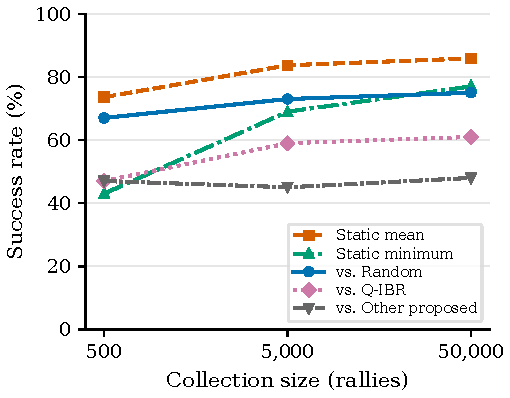
\includegraphics[width=\linewidth]{Figures/ablation_training_size.pdf}
\caption{$\alpha$-potential data-collection ablation with a logarithmic rally-count axis.}
\label{fig:datavolume}
\end{minipage}\hfill
\begin{minipage}[t]{0.48\linewidth}
\centering
\vspace{0pt}
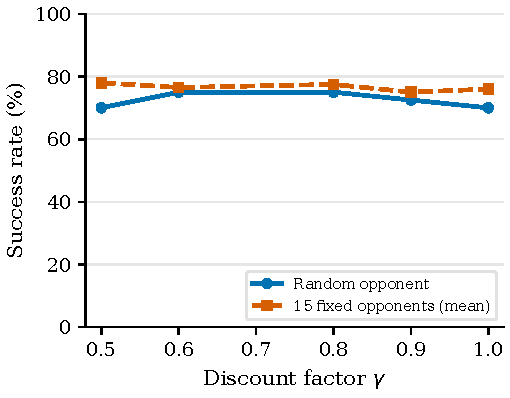
\includegraphics[width=\linewidth]{Figures/ablation_discount_factor.pdf}
\caption{$\alpha$-potential discount-factor ablation across four opponent metrics.}
\label{fig:discountfactor}
\end{minipage}
\end{figure}

\section{Conclusion}
\label{sec:conclusion}
We presented an attacker--defender framework for competitive robot table tennis, with decisions at net crossings and shared execution controllers. A learned $\alpha$-potential selects among fifteen first-exchange action profiles, while PPO self-play learns state-dependent strategies. Potential planning achieves the strongest static-opponent results, while argmax self-play attains higher win rates against Random and Q-IBR. Empirical response gains separately assess equilibrium quality. Additional training data improve fixed-opponent performance. This shared formulation supports direct comparison of equilibrium-aware planning and reinforcement learning.

% Flush main-text floats before the references.
\clearpage
% The jmlr class selects plainnat automatically.
\bibliography{references}

% Start supplementary material on a fresh page after all references.
\clearpage
\appendix
\section{Proof of the Equilibrium Approximation}
\label{app:potentialproof}
For the first-exchange policy family, the initial roles and random continuation rule are fixed while each player varies its initial action. We prove Proposition~\ref{prop:potential} under these conditions.
\begin{proof}
For every player $i$ and admissible deviation $\theta^i$, Equation~\eqref{eq:alphapotential} gives
\begin{align*}
 V^i(x,\theta^i,\theta^{*,-i})-V^i(x,\theta^*)
 &\leq\Phi(x,\theta^i,\theta^{*,-i})-\Phi(x,\theta^*)+\alpha\\
 &\leq\lambda+\alpha.
\end{align*}
\end{proof}



\section{Error Propagation in Two-Stage Potential Learning}
\label{app:potentialerrors}
\paragraph{Anchored labels and composite regression.}
Equation~\eqref{eq:potentialtraining} fixes $p_{x,\theta_{\mathrm{ref}}}^\star=0$ for every sampled state, with $\theta_{\mathrm{ref}}=(1,1)$ corresponding to array entry $[0,0]$. Adding a nonzero constant violates this constraint, so the labels share a consistent origin across states. The remaining fourteen values are free real variables subject to the discrepancy inequalities. The anchor removes the additive ambiguity without requiring the rest of the optimal table to be unique. Labels retain this reference value; no mean centering is applied.

Write $f_x(\theta)=\Phi_\varphi(x,\theta)$ and define $\Delta_{\theta,\theta'} f_x=f_x(\theta)-f_x(\theta')$, with the same difference operator for $p_x^\star$. The regression terms are
\begin{equation}
\begin{aligned}
 \mathcal L_{\mathrm{abs}}
 &=\mathbb E_{x,\theta}\big[(f_x(\theta)-p_{x,\theta}^\star)^2\big],\\
 \mathcal L_{\mathrm{LPdiff}}
 &=\mathbb E_{x,(\theta,\theta')\in\mathcal P_x}
   \big[(\Delta_{\theta,\theta'} f_x-\Delta_{\theta,\theta'}p_x^\star)^2\big],\\
 \mathcal L_{\mathrm{Qdiff}}
 &=\mathbb E_{x,(i,\theta,\theta^{i\prime})\in\mathcal D_x}
   \big[e_\varphi(x,i,\theta,\theta^{i\prime})^2\big].
\end{aligned}
 \label{eq:potentiallosses}
\end{equation}
These expectations denote empirical averages over training states, profiles, and pairs. The LP-difference loss uses $\mathcal P_x=\Theta\times\Theta$, covering all 225 ordered pairs of the fifteen profiles. The Q-difference term uses unilateral deviations and the frozen Q-values in Equation~\eqref{eq:potentialresidual}. Both difference-loss weights default to one, as shown in Equation~\eqref{eq:potentialregression}. The absolute term fits the anchored values, while the difference terms fit their strategic variations. In particular, the reference output is trained toward zero through $\mathcal L_{\mathrm{abs}}$, without an output-layer constraint enforcing it exactly.

\paragraph{Approximation error.}
Fix a sampled state $x$ and its initial role assignment. Suppose the Q-network and potential network satisfy
\begin{equation}
\begin{aligned}
 \max_{i,\theta}\big|\widehat V^i_{\nu_i}(x,\theta)-V^i(x,\theta)\big|&\leq\beta_x,\\
 \max_\theta\big|\Phi_\varphi(x,\theta)-p_{x,\theta}^\star\big|&\leq\varepsilon_x.
\end{aligned}
 \label{eq:estimationerrors}
\end{equation}
For any unilateral deviation, the triangle inequality gives
\begin{equation}
\begin{aligned}
 \big|&\Phi_\varphi(x,\theta)-\Phi_\varphi(x,\theta^{i\prime},\theta^{-i})\\
 &-\big[V^i(x,\theta)-V^i(x,\theta^{i\prime},\theta^{-i})\big]\big|
 \leq y_x^\star+2\beta_x+2\varepsilon_x.
\end{aligned}
 \label{eq:twostageerror}
\end{equation}
The LP contributes $y_x^\star$, the two Q-estimation errors contribute at most $2\beta_x$, and the two regression errors contribute at most $2\varepsilon_x$. A uniform bound across initial states supplies the $\alpha$ required by Proposition~\ref{prop:potential}; adding an online optimization gap $\lambda$ gives the corresponding $(\alpha+\lambda)$-equilibrium guarantee. The composite regression objective in Equation~\eqref{eq:potentialregression} uses empirical MSE terms, while this guarantee uses uniform error. Empirical unilateral response gains assess the deployed feedback policies.

\section{Self-Play and Potential-Based Policy Representations}
\label{app:selfplay}
Only the actor head in Equation~\eqref{eq:rlheads} corresponding to the active role selects an action. The actor receives the same physical information available to the potential-based planner, without access to the opponent's newly sampled action. The actor conditions its strategic probabilities on each new state throughout the rally. In contrast, Equation~\eqref{eq:firstexchangepolicy} evaluates an initial action followed by random continuation; the deployed potential planner recomputes that initial action at every exchange.

\paragraph{Training objective and opponent updates.}
We train each player to maximize its discounted point utility using proximal policy optimization (PPO) with a learned value baseline \citep{schulman2017ppo}. PPO optimizes a clipped probability-ratio surrogate using advantage estimates from the critic.
We alternate learner updates while holding the opponent fixed within each update round. We maintain a pool of frozen opponent snapshots and sample one at the beginning of each rally, retaining it for the rally's duration. This exposes the learner to earlier strategies as well as recent opponents. Both players experience attack and defense transitions, and rewards and value targets follow their player identities through role switches. A critic estimates the player's return, and entropy regularization encourages exploration of target and preparation choices. Terminal rollouts use the observed point outcome. For rollouts truncated before termination, we bootstrap the remaining return from the critic.


% \section{Human-Play Processing and Position-Conditioned Comparison}
% \label{app:humananalysis}
% \paragraph{Human strategy and video-based analysis.}
% Human table tennis strategies have been inferred through inverse reinforcement learning \citep{muelling2014strategies}, while TTNet and LATTE-MV support video analysis and anticipation \citep{voeikov2020ttnet,etaat2025latte}. This appendix compares human shot-placement distributions with simulated play.

% \label{sec:resultshuman}
% We compare learned strategies with human gameplay reconstructed from monocular videos using LATTE-MV \citep{etaat2025latte}.

% \paragraph{Position-conditioned return heatmaps.}
% We extract player locations, racket-contact events, and returned-ball landing locations from human table tennis videos, using calibrated table coordinates and exchange segmentation \citep{etaat2025latte,voeikov2020ttnet}. We mark exchanges at net crossings and express them in a common attacker-oriented frame so that left and right have the same meaning across players, videos, and simulation. At the matched net-crossing decision epoch, we assign the attacker and opponent to lateral bins $s^{\attack},s^{\defend}\in\{L,C,R\}$. We analyze all nine position combinations, including attacker-left/opponent-left and attacker-left/opponent-right. We assign valid first-bounce locations on the opponent's half to the five return regions using a fixed coordinate partition. Table~\ref{tab:humancorrelation} presents the human--model comparison.

% For each context $s=(s^{\attack},s^{\defend})$, we estimate
% \begin{equation}
%   h_{\mathrm{human}}(k\mid s)=
%   \frac{n_{\mathrm{human}}(k,s)}
%        {\sum_{j=1}^{5}n_{\mathrm{human}}(j,s)},
%   \quad k\in\mathcal{K},
%   \label{eq:humanheatmap}
% \end{equation}
% where $n_{\mathrm{human}}(k,s)$ counts observed returns in target region $k$ and context $s$. We apply the same procedure to realized landing locations from each proposed method. Table~\ref{tab:humancorrelation} summarizes Pearson correlations and Jensen--Shannon divergences between the human and model distributions. Correlation is undefined for a constant distribution, so such cases are reported separately. This comparison characterizes how the learned policies and random baseline distribute returns relative to human play in each position context. The analysis concerns conditional shot-placement patterns within the shared target representation.

% \begin{table}[t]
% \centering
% \small
% \begin{tabular}{lccccccc}
% \toprule
% Context & Human returns & $\rho_{\alpha}$ & $\rho_{\mathrm{RL}}$ & $\rho_{\mathrm{rand}}$ & $\mathrm{JS}_{\alpha}$ & $\mathrm{JS}_{\mathrm{RL}}$ & $\mathrm{JS}_{\mathrm{rand}}$\\
% \midrule
% $(L,L)$ & \resultblank & \resultblank & \resultblank & \resultblank & \resultblank & \resultblank & \resultblank\\
% $(L,C)$ & \resultblank & \resultblank & \resultblank & \resultblank & \resultblank & \resultblank & \resultblank\\
% $(L,R)$ & \resultblank & \resultblank & \resultblank & \resultblank & \resultblank & \resultblank & \resultblank\\
% $(C,L)$ & \resultblank & \resultblank & \resultblank & \resultblank & \resultblank & \resultblank & \resultblank\\
% $(C,C)$ & \resultblank & \resultblank & \resultblank & \resultblank & \resultblank & \resultblank & \resultblank\\
% $(C,R)$ & \resultblank & \resultblank & \resultblank & \resultblank & \resultblank & \resultblank & \resultblank\\
% $(R,L)$ & \resultblank & \resultblank & \resultblank & \resultblank & \resultblank & \resultblank & \resultblank\\
% $(R,C)$ & \resultblank & \resultblank & \resultblank & \resultblank & \resultblank & \resultblank & \resultblank\\
% $(R,R)$ & \resultblank & \resultblank & \resultblank & \resultblank & \resultblank & \resultblank & \resultblank\\
% \bottomrule
% \end{tabular}
% \caption{Position-conditioned human comparison. The correlations $\rho$ and Jensen--Shannon divergences $\mathrm{JS}$ compare realized landing distributions against human play. The subscript $\mathrm{rand}$ denotes the random baseline.}
% \label{tab:humancorrelation}
% \end{table}

\section{Low-Level Execution Controllers}
\label{app:execution}
\paragraph{Exchange timing and role switching.}
An exchange begins when the incoming ball crosses the net toward the current attacker. This crossing marks the strategic decision epoch: the state is sampled, the attacker selects a return target, and the defender selects a preparation position. The execution controllers then track these choices while the attacker returns the ball and the defender prepares. When the returned ball crosses the net and the rally continues, the next exchange begins with $(\iota_{t+1},\jmath_{t+1})=(\jmath_t,\iota_t)$. A rally that terminates before the next crossing transitions directly to a terminal state.

The previous defender now receives the ball and becomes the attacker. An invalid incoming shot or a failed return terminates the rally and assigns its point outcome. The initialization specifies the first incoming ball and the corresponding attacker, allowing rally strategy to be studied without prescribing a separate serving controller. Strategic epochs therefore index exchanges, while the simulator and robot controllers execute at finer physical time steps.

\paragraph{Joint state.}
The state includes the variables needed to predict the consequences of both players' choices: $x_t=(b_t,z_t^1,z_t^2,\iota_t,\ell_t)$, where $b_t=(p_t^b,v_t^b,\omega_t^b)$.
Here $p_t^b,v_t^b,\omega_t^b\in\R^3$ are the ball position, linear velocity, and angular velocity. The robot state $z_t^i$ contains its gantry position and joint angles, their velocities, and any actuator or controller state required for a Markov description. Racket poses follow from the robot kinematics. The discrete variable $\ell_t$ records rally status, including the last contact, bounce information, and terminal outcome. Keeping both robot states in $x_t$ preserves the effect of previous recovery and preparation motions on future returns.

\paragraph{Controller interface.}

The strategic actions are executed by the fixed attack and preparation controllers described in Section~\ref{sec:game}. The attack controller receives the current physical state and the selected landing target, and commands the gantry and arm to return the incoming ball toward that target. The preparation controller receives the selected ready configuration and moves the robot toward it while the opponent executes its return. Both controllers use state feedback at the simulator's physical time steps.

MuJoCo advances the ball and robot dynamics and resolves racket, table, and net interactions. The returned ball's net crossing switches the strategic roles; a failed return or an invalid shot terminates the rally. The same execution controllers and physical parameters are used across all strategic methods, so the comparison isolates the selection of return targets and preparation positions.

\subsection{Reinforcement Learning for Racket-Pose Tracking}
\label{app:trackertraining}
The low-level controller is pretrained with PPO \citep{schulman2017ppo} on a single-robot racket-pose tracking task. The robot consists of a seven-joint KUKA iiwa arm and a two-axis gantry. The training environment supplies a sequence of desired racket poses, and the policy learns continuous commands that reduce pose error. This pretraining is independent of the strategic self-play policies: shot placement enters the tracker through its desired pose, while the tracker reward measures execution quality.

\paragraph{Observations and actions.}
The observation has 68 entries: nine robot positions, nine velocities, three position errors, four relative quaternion components, seven desired pose components, and four previous actions with nine entries each. The relative rotation is $R_s^\star R_s^\top$, where $R_s$ and $R_s^\star$ denote the current and desired racket orientations. The action history stores commands scaled by 0.1. The desired position and quaternion provide absolute target information in addition to the pose errors.

Each policy action $a_s\in[-1,1]^9$ contains two gantry commands followed by seven arm commands. With the training configuration, the commands are applied as
\begin{equation}
\begin{aligned}
 g_s^+&=\operatorname{clip}_{\mathcal G}\big(g_s+0.01a_s^{1:2}\big),\\
 u_s^{\mathrm{arm}}&=q_s^{\mathrm{arm}}+0.1a_s^{3:9},
 \qquad \mathcal G=[-1.2,-0.3]\times[-1,1].
\end{aligned}
 \label{eq:trackeraction}
\end{equation}
Here $g_s$ is the gantry position and $u_s^{\mathrm{arm}}$ is the arm position-control target. Gantry coordinates are updated directly before the physics step; the arm uses position servos with proportional and velocity gains of 2000 and 200. Each action advances one MuJoCo step of 0.01\,s, giving a 100\,Hz control rate.

\paragraph{Target sampling and curriculum.}
Target positions are sampled independently in robot-local coordinates from $[-0.5,0.2]$\,m longitudinally, $[-1.1,1.1]$\,m laterally, and $[0.75,1.05]$\,m vertically. Target orientations use a forward-facing racket normal with bounded random tilt and roll perturbations. Reaching a target resamples the desired pose within the same episode. Episodes contain at most 1000 simulator steps, corresponding to 10\,s; the first two episodes use randomized initial step counters.

Define the weighted pose error
\begin{equation}
 C_s=10\|p_s-p_s^\star\|_2
     +10\operatorname{angle}\big(R_s^\star R_s^\top\big),
 \label{eq:trackerposeerror}
\end{equation}
with rotation angle in radians. A target is resampled when $C_s<\tau(n)$, where
\begin{equation}
 \tau(n)=1+1.5\exp\!\left(-\frac{n}{46{,}875}\right)
 \label{eq:trackercurriculum}
\end{equation}
and $n$ counts cumulative control steps in each training environment. The tolerance therefore decreases from 2.5 toward 1.0. Evaluation fixes the tolerance at 1.0.

\paragraph{Tracking reward.}
Between target changes, PPO receives the reduction in weighted pose error, together with an action-effort penalty. At the action scales in Equation~\eqref{eq:trackeraction}, the implemented reward is
\begin{equation}
 r_s^{\mathrm{track}}=C_{s-1}-C_s-\frac{1}{90}\|a_s\|_1.
 \label{eq:trackerreward}
\end{equation}
The implementation applies an effort penalty of $\|0.1a_s\|_1/9$, yielding the coefficient in Equation~\eqref{eq:trackerreward}. On a target-resampling step, the returned reward is set to zero and the pose-error baseline is recomputed for the new target. Observations are assembled before resampling, so the newly drawn target enters the following observation. This shaping reward trains racket execution separately from the competitive point utility in Equation~\eqref{eq:reward}.

\paragraph{PPO training configuration.}
The actor and critic each have three hidden layers with widths $512$, $256$, and $128$, using ELU activations. Training uses 256 vectorized environments, 50 rollout steps per environment, and five PPO optimization epochs per rollout. The learning rate is $5\times10^{-4}$ and the discount factor is 0.99. Table~\ref{tab:trackertraining} lists the configured training settings. Although the requested minibatch size is 32,768, each rollout contains only $256\times50=12,800$ transitions; each optimization epoch therefore uses one minibatch containing 12,800 transitions. Deterministic evaluation averages ten episodes every 2000 vectorized control steps, and the checkpoint with the highest mean evaluation return is retained.

\begin{table}[tbp]
\centering
\small
\begin{tabular}{ll}
\toprule
Setting & Value\\
\midrule
Actor / critic hidden layers & $(512,256,128)$ / $(512,256,128)$\\
Activation & ELU\\
Vectorized environments & 256\\
Rollout steps per environment & 50\\
Transitions per rollout & 12,800\\
Requested / effective minibatch & 32,768 / 12,800\\
Optimization epochs per rollout & 5\\
Learning rate & $5\times10^{-4}$\\
Discount factor & 0.99\\
Configured training budget & $10^8$ environment transitions\\
Evaluation interval & 2000 vectorized steps (512,000 transitions)\\
Evaluation episodes & 10, deterministic actions\\
\bottomrule
\end{tabular}
\caption{Low-level pose-tracker PPO configuration. The effective minibatch is limited by the number of transitions in a rollout.}
\label{tab:trackertraining}
\end{table}

\paragraph{Deployment in the competitive environment.}
A ballistic targeting module predicts candidate interception positions and reflected ball velocities, then chooses a racket normal that minimizes predicted landing error relative to the strategic return target. The resulting position and orientation are supplied to the frozen pose tracker. The same checkpoint is evaluated deterministically for both robots using their local robot states, target-pose errors, and action histories; their nine-dimensional commands are concatenated into the two-robot action. Thus, strategic target selection, analytic racket-pose generation, and learned pose tracking form successive stages of the execution interface.

\end{document}
